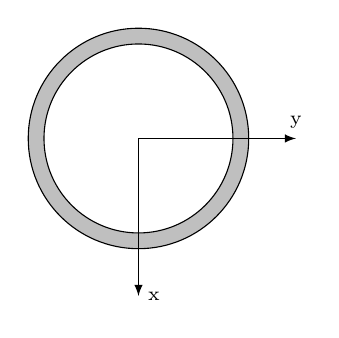
\begin{tikzpicture}
%linee guida
%\foreach \x in {0,1,...,15}
%   \draw [help lines] (\x,0) node [below,%
%          font=\footnotesize] {$\x$} -- (\x,15);
%\foreach \y in {0,1,...,15}
%   \draw [help lines] (0,\y) node [left,%
%          font=\footnotesize] {$\y$} -- (15,\y);

% InternalRadius, 0.012
% ExternalRadius, 0.014
\draw[fill=lightgray] (7.5,7.5) circle (14mm);
\draw[fill=white] (7.5,7.5) circle (12mm);
%reference system
\draw[-latex] (7.5,7.5)--(7.5,5.5)node[right]{\scriptsize x};
\draw[-latex] (7.5,7.5)--(9.5,7.5)node[above]{\scriptsize y};

%% quote track
 \dimline    [color=gray,
 			  label style={above=0.1ex},
                % line style={thick},
                %extension start style={gray,thin},
                %extension end style={gray,thin},
                extension start length=1.75cm,
                extension end length=1.75cm
                ]{(7.5-1.2,9.25)}{(7.5+1.2,9.25)}{$12$};
                
\dimline    [color=gray,
			 label style={above=0.1ex},
                % line style={thick},
                %extension start style={gray,thin},
                %extension end style={gray,thin},
                extension start length=2.5cm,
                extension end length=2.5cm
                ]{(7.5-1.4,10)}{(7.5+1.4,10)}{$14$};
\end{tikzpicture}